\graphicspath{{figures/analysis/}}
\chapter{Data Analysis}\label{ch:data_anal}
To be able to develop a solution which is able to detect which type of occlusion and the location of it, some analysis of the data is necessary. This is also done to determine how many and which kind af categories of occlusion there is.

The data primarily used, is a 60 second video with three zebrafish recorded at 50 \gls{fps}.

\section{Fish Shapes}
Even a single a fish is able to twist into many different shapes, according to \cite{Kalueff2013} zebrafish has an extensive catalogue of behavioural patterns, which are also based on different contortions of the body. The main shapes of a single fish are shown in \autoref{fig:single_shape}. The shapes shown are only the ones seen from the top view of an aquarium.

\begin{figure}[H]
	\centering
	\begin{subfigure}[b]{0.3\textwidth}
		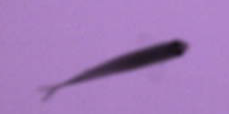
\includegraphics[width=\textwidth]{straight}
		\caption{Zebrafish lying completely straight}
		\label{fig:straight_fish}
	\end{subfigure}
	\begin{subfigure}[b]{0.3\textwidth}
		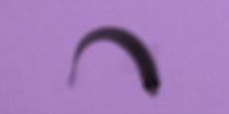
\includegraphics[width=\textwidth]{c-shape}
		\caption{Zebrafish creating a C shape}
		\label{fig:c-shape_fish}
	\end{subfigure}
	\begin{subfigure}[b]{0.3\textwidth}
		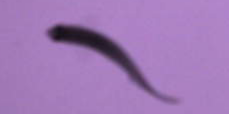
\includegraphics[width=\textwidth]{s-shape}
		\caption{Zebrafish creating an S shape}
		\label{fig:s-shape_fish}
	\end{subfigure}
\caption{Different shapes a zebrafish makes from a top view, also described by \cite{Kalueff2013}}
\label{fig:single_shape}
\end{figure}

\cite{Kalueff2013} states that the C-shape is made as starting movement to propel itself forward, often in order to escape or because the fish is startled. The bending into a C-shape, can also be caused by the fish turning. The S-shape is made for the same reasons as the C-shape, to propel the fish forward.\\

When two fish are touching or crossing each other in any way, they create multiple new shapes.

\subsection{Touching}
When two fish are touching they in general create three different kind of shapes. They will either be elongating one another, creating one single long object. This can be either head-to-head or head-to-tail. Both examples are shown in \autoref{fig:elongation}. When touching head-to-tail it is most often seen as courtship between a male and a female fish \citep{Kalueff2013}.

\begin{figure}[H]
	\centering
	\begin{subfigure}[b]{0.47\textwidth}
		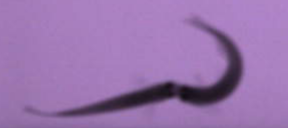
\includegraphics[width=\textwidth]{headhead}
		\caption{Head-to-head elongation}
		\label{fig:headhead}
	\end{subfigure}
	\begin{subfigure}[b]{0.47\textwidth}
		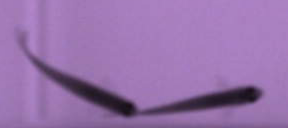
\includegraphics[width=\textwidth]{headtail}
		\caption{Head-to-tail elongation}
		\label{fig:headtail}
	\end{subfigure}
\caption{The two touching possibilities creating an elongation}
\label{fig:elongation}
\end{figure}

Two fish touching is done in all kinds of positions and angles. When touching end-to-end but at a tighter angle, two fish tend to create a V-shape. In the beginning and end of a crossing or when touching the head or tail to the middle of the body of another fish, a T-shape is created. Examples of both shapes are shown in \autoref{fig:TandV}.

\begin{figure}[H]
	\centering
	\begin{subfigure}[b]{0.47\textwidth}
		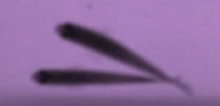
\includegraphics[width=\textwidth]{v-shape}
		\caption{V-shape created by two fish touching tails}
		\label{fig:v-shape}
	\end{subfigure}
	\begin{subfigure}[b]{0.47\textwidth}
		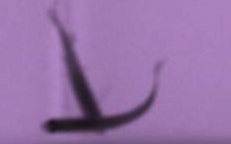
\includegraphics[width=\textwidth]{t-shape}
		\caption{T-shape example}
		\label{fig:t-shape}
	\end{subfigure}
\caption{Examples of T- and V-shape}
\label{fig:TandV}
\end{figure}

\subsection{Above and Below}
More complete occlusions often happen when one fish is above the other. The higher the water goes in an aquarium, the more likely the fish will be to swim above one another, as this gives them more space to move around in. There is mainly two different occlusions happening in this instance, which is two fish creating a cross, or one fish almost completely occluding the other.

The crossing can happen in multiple different angles. A crossing occlusion is defined as two fish creating an X-shape. Examples of different crosses are shown in \autoref{fig:cross}. 

\autoref{fig:crossWide} shows a crossing occlusion, which is close to being an \textit{on-top} occlusion, but will be defined as a cross due to the head and tails being separated.

\begin{figure}[H]
	\centering
	\begin{subfigure}[b]{0.3\textwidth}
		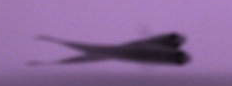
\includegraphics[width=\textwidth]{crossWide}
		\caption{Cross occlusion at a wide angle}
		\label{fig:crossWide}
	\end{subfigure}
	\begin{subfigure}[b]{0.3\textwidth}
		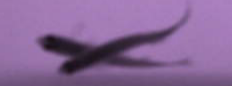
\includegraphics[width=\textwidth]{crossSemi}
		\caption{Cross occlusion at a semi-wide angle}
		\label{fig:crossSemi}
	\end{subfigure}
	\begin{subfigure}[b]{0.3\textwidth}
		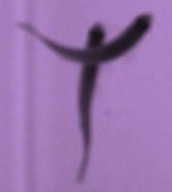
\includegraphics[width=\textwidth]{crossRight}
		\caption{Cross occlusion at an almost right angle}
		\label{fig:crossRight}
	\end{subfigure}
	\caption{Different cross occlusions}
	\label{fig:cross}
\end{figure}

The on-top occlusions is when one fish is at least somewhat straight on top of another fish. This kind of occlusions can at times be a shorter kind of elongation, when the head of the top fish is further in on the body of the bottom fish. Examples of op-top occlusion are shown in \autoref{fig:onTop}.

\begin{figure}[H]
	\centering
	\begin{subfigure}[b]{0.47\textwidth}
		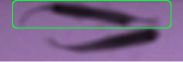
\includegraphics[width=\textwidth]{onTop}
		\caption{Straight on top occlusion}
		\label{fig:onTopFull}
	\end{subfigure}
	\begin{subfigure}[b]{0.47\textwidth}
		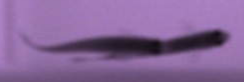
\includegraphics[width=\textwidth]{onTopMid}
		\caption{Head on top of middle of bottom fish}
		\label{fig:onTopMid}
	\end{subfigure}
	\caption{On-top occlusions by two fish}
	\label{fig:onTop}
\end{figure}

\subsection{Other Occlusions}
Besides the five previously mentioned types of occlusions, several other occlusions occur which are harder to classify as they do not fall into any specific category. Due to this, a category named \textit{other} is created as well. Some examples of these kinds of occlusions are shown in \autoref{fig:other}.

\begin{figure}[H]
	\centering
	\begin{subfigure}[b]{0.3\textwidth}
		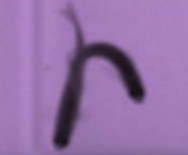
\includegraphics[width=\textwidth]{otherR}
		\caption{Example of occlusion categorised as \textit{other}}
		\label{fig:otherR}
	\end{subfigure}
	\begin{subfigure}[b]{0.3\textwidth}
		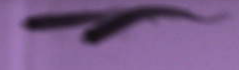
\includegraphics[width=\textwidth]{otherTop}
		\caption{Example of occlusion categorised as \textit{other}}
		\label{fig:otherTop}
	\end{subfigure}
	\begin{subfigure}[b]{0.3\textwidth}
		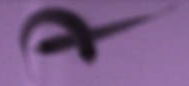
\includegraphics[width=\textwidth]{otherP}
		\caption{Example of occlusion categorised as \textit{other}}
		\label{fig:otherP}
	\end{subfigure}
	\caption{Different \textit{other} occlusions}
	\label{fig:other}
\end{figure}

Occlusions occurring with all three fish are also categorised as other, as none of these fall into the defined categories, but are still occlusions.\todo{Forklar og begrund hvorfor der primært fokuseres på okklusioner med 2 fisk indblandet,og giv eksempler på det.}

\section{Occlusion Frequency}
The occlusions happen with different frequencies, but some clearly occur more often than others:

\begin{figure}[H]
	\centering
	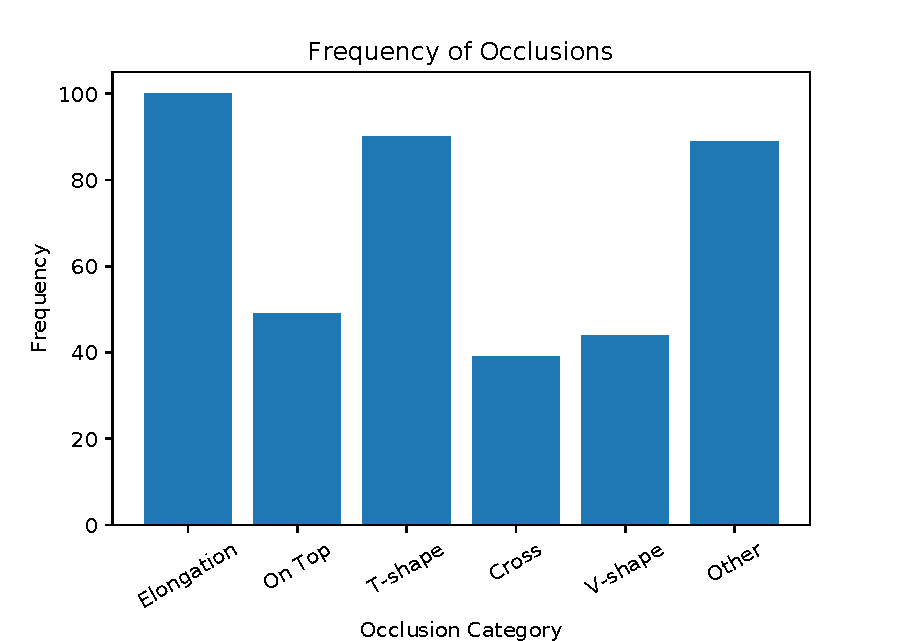
\includegraphics[width=0.8\textwidth]{occlFreq}
	\caption{Frequency of the different types of occlusions}
	\label{fig:occlFreq}
\end{figure}

\autoref{fig:occlFreq} shows that elongation is the most frequently occurring occlusion, together with the T-shape and other types of occlusions. In total $ 411 $ occlusions occur out of $ 3000 $ frames, which is $13.7\%$.